\chapter{Einleitung}

%----------------------------------------------------------------------------------------

Die folgenden Kapitel beschreiben den Prozess, der nötig war um das Schloss
Rapperswil mittels Luftbilder als 3D-Modell zu rekonstruieren. Wir gehen hier
nicht auf die Evaluation der genutzten Software ein, dies folgt im nächsten Teil
dieser Dokumentation.

%----------------------------------------------------------------------------------------

\section{Erfassung des Schlosses mit Kamera-Drohne}

Um Fotos des Schlosses von allen Winkeln zu erstellen, braucht man ein
ferngesteuertes Flugobjekt wie z.~B. einen Multikopter. In unserem Fall wurden
die Fotos von Michael Suter (\url{http://lightmoment.ch/}) erstellt, der einen
Quadrokopter besitzt und daran freundlicherweise seine Piloten-Fähigkeiten unter
Beweis gestellt hat.

\subsection{Materialliste}

\begin{itemize}
	\item Quadrokopter: \textit{Team BlackSheep Discovery
		Pro}\footnote{\url{http://www.team-blacksheep.com/products/prod:discopro}}
	\item Kamera: \textit{GoPro Hero 4 Black}\footnote{\url{https://gopro.com/}}
	\item GPS Tracker: \textit{Fairphone
		FP1}\footnote{\url{https://www.fairphone.com/}} mit
		\textit{GeoTracker}
		App\footnote{\url{https://play.google.com/store/apps/details?id=com.ilyabogdanovich.geotracker}}
\end{itemize}

\subsection{Vorgehen}

Die maximale Flugzeit pro Akku beträgt 10--15 Minuten. Wir hatten zwei geladene
Akkus dabei und erreichten somit eine Flugzeit von 20--30 Minuten.

Die GoPro Kamera hatten wir so eingestellt, dass sie zwei mal pro Sekunde ein
Bild machte. Daraus ergaben sich dann etwa 2700 Fotos, was ca. 5.3 GiB
Bildmaterial entspricht.

Um Bewegungs-Unschärfe bei den Bildern zu vermeiden, ist es wichtig, dass der
Multikopter über eine Kamera-Stabilisierung verfügt. Dies ist bei der genutzten
TBS Discovery mit einem Gimbal (gyroskopische Mehrachsen-Stabilisierung)
gegeben.

Zur Aufzeichnung der GPS-Koordinaten haben wir ein Smartphone mit einer GPS
Tracking App auf dem Quadrokopter befestigt. Das ist nicht sehr professionell,
hat aber gut funktioniert.

\begin{figure}[p]
	\centering
	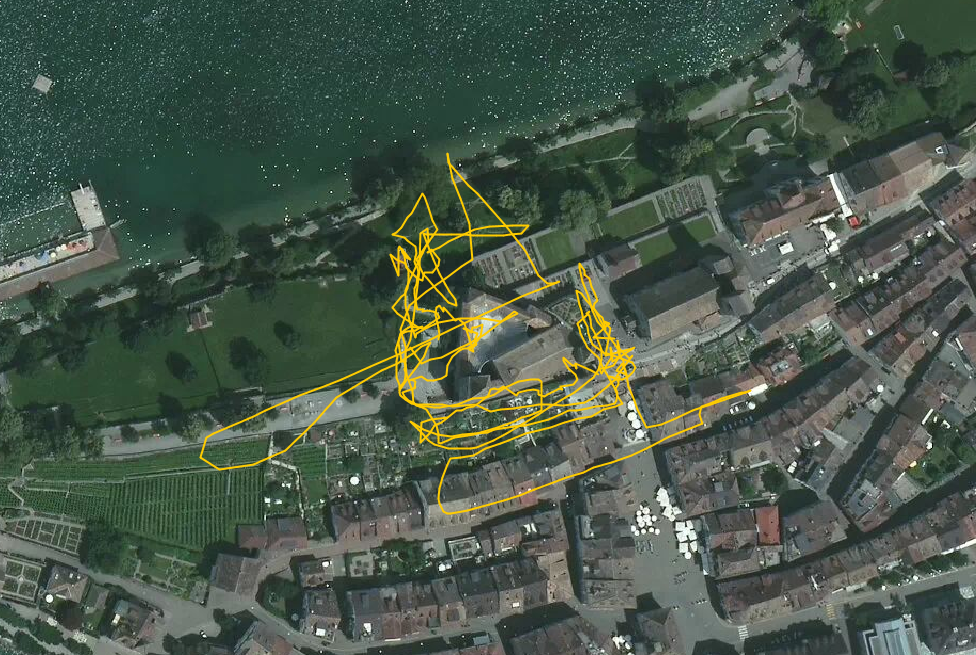
\includegraphics[width=\textwidth]{images/gpstrace_satellite.png}
	\caption{GPS Trace des Quadrokopters während der Erfassung.\\Bildmaterial:
		\copyright{} Bing Maps}
	\label{img:gpstrace-satellite}
\end{figure}

\begin{figure}[p]
	\centering
	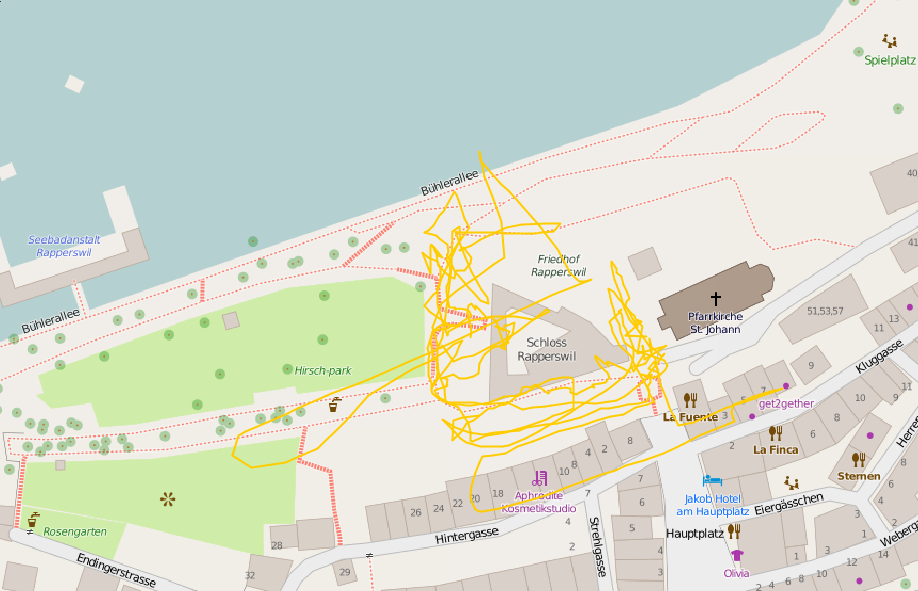
\includegraphics[width=\textwidth]{images/gpstrace_mapnik.png}
	\caption{GPS Trace des Quadrokopters während der Erfassung.\\Bildmaterial:
		\copyright{} OpenStreetMap Contributors}
	\label{img:gpstrace-mapnik}
\end{figure}

\subsection{Bildqualität}

Die GoPro Kamera ist für Sportaktivitäten entwickelt worden und hat daher ein
Weitwinkel-Objektiv ("<Fisheye">) eingebaut. Dies ist bestens geeignet um
beispielsweise beim Skifahren einen guten Überblick zu bewahren, für die
Rekonstruktion ist es aber eher nachteilig.

Ein weiterer Faktor ist die Kompression. Um viele Bilder auf der SD-Karte
speichern zu können, werden die JPEG-Bilder stark komprimiert. Die daraus
entstehenden JPEG-Artefakte können die Feature-Detection stören.

Idealerweise würde man daher zur Erfassung eine Spiegelreflex-Kamera mit
neutralem 35mm Objektiv verwenden und alle Bilder im RAW-Format abspeichern.
Diese können dann mit entsprechender Software ohne verlustbehaftete Kompression
in ein für die Photogrammetrie\-/Software nutzbares Format umgewandelt werden.

In unserem Fall waren wir aber durch die Tragfähigkeit des Quadrokopters
eingeschränkt und haben uns stattdessen dafür entschieden, die Bilder am
Computer mithilfe eines Linsenprofils zu entzerren (TODO Referenz). Inzwischen
gibt es allerdings sogar Photogrammetrie\-/Programme welche die GoPro
Linsenprofile direkt unterstützen. Nichtsdestotrotz gibt es sicher Kameras
welche besser für solche Aufgaben geeignet sind als die GoPro.

\subsection{Learnings}

\begin{itemize}
	\item Die Jahreszeit war an sich gut gewählt, da die Bäume im Winter nicht
		belaubt sind, wodurch die Sicht auf das Schloss nicht eingeschränkt wird.
	\item Nachteilig war jedoch der Schnee auf den Dächern. Er überdeckte die
		Dachziegel und führte so bei der Feature-Erkennung zu schlechteren
		Ergebnissen.
	\item Die GoPro hat eine äusserst starke Verzerrung. 
\end{itemize}
